\documentclass[]{standalone}

\usepackage{amsmath}
\usepackage{amsfonts}
\usepackage{amssymb}
\usepackage{graphicx}
\usepackage{tikz}
\usepackage{import}
\usepackage[subpreambles=true]{standalone}

\usepackage{tikz}
\usepackage{tikz-3dplot}
\usepackage{tikz_utils}

\usetikzlibrary{calc}
\usetikzlibrary{positioning}
\usetikzlibrary{patterns}
\usetikzlibrary{decorations,backgrounds}

\begin{document}

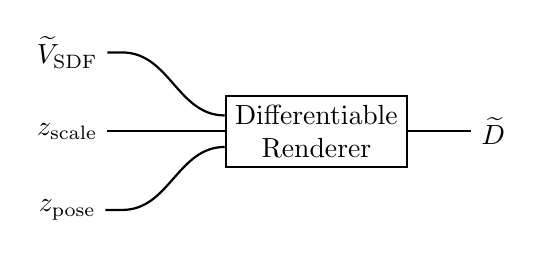
\begin{tikzpicture}[scale=1]

    % \draw[thick] (2,0,0)--(2.8,0,0);
    % \draw[thick] (2.8,1,0) -- (3.1,1,0) -- (3.1,-1,0) -- (2.8,-1) -- cycle;

    \node (sdf_volume) at (0,1) {$\widetilde{V}_\mathrm{SDF}$} ;
    \node (z_scale) at (0,0)  {$z_\mathrm{scale}$};
    \node (z_pose) at (0,-1)  {$z_\mathrm{pose}$};
    \node [draw=black, thick, align=center, anchor=west] (diff_rend) at (2,0) {Differentiable\\Renderer};
    % \draw[thick] (z_scale.east) -- (diff_rend.west);

    \draw[thick] (sdf_volume.east) -- (0.7,1) to[out=0,in=180] ($(diff_rend.west)+(0,0.2)$);
    \draw[thick] (z_pose.east) -- (0.7,-1)  to[out=0,in=180] ($(diff_rend.west)+(0,-0.2)$);
    \draw[thick] (z_scale.east) -- (diff_rend.west);
 
    \draw[thick] (diff_rend.east) -- ++(0.8,0) node[right] {$\widetilde{D}$};
    
\end{tikzpicture}
\end{document}